\section{Algoritmo parallelo}

La popolazione di cellule è modellata tramite un array, una delle strutture
dati più adatte ad essere parallelizzate su GPU, dato che è possibile
demandare la computazione di ogni elemento dell'array ad uno specifico thread.
Sia la creazione che la simulazione della proliferazione fanno uso solamente di
array unidimensionali, dunque il problema si riduce all'implementazione di un
algoritmo in grado di massimizzare il parallelismo necessario alla computazione
dell'insieme di array atto a portare a termine la simulazione. 

% Descrizione della creazione della popolazione iniziale partendo dal file
% dell'istogramma di partenza
\subsection{Creazione della popolazione iniziale}

L'istogramma $H(0)$ che riporta i valori di fluorescenza con la rispettiva
frequenza è salvato su un file di testo che deve essere letto in modo
sequenziale. Una volta letto l'intero file sarà stato creato un array i cui
elementi saranno le coppie di valori $(\varphi_{i}, \psi_{i})$.
Ora che è nota la frequenza $\psi_{i}$ per ogni fluorescenza $\varphi_{i}$,
è possibile invocare l'esecuzione di un Kernel per ogni coppia di
valori 
in modo tale che ogni thread si occupi di generare una cellula avente
$\varphi_{i}$ valore di fluorescenza come rappresentato in figura
\ref{fig:population-creation}.
\\
\begin{figure}[t]
    \centering
    \begin{tikzpicture}
        \pgftransparencygroup
        \nodes{(\varphi_{i}, \psi_{i})}
        \endpgftransparencygroup
        \pgftransparencygroup
        \hiddennodes{$\longrightarrow$}
        \endpgftransparencygroup
        \pgftransparencygroup
        \nodes{\varphi_{i}, \varphi_{i}}
        \endpgftransparencygroup
        \pgftransparencygroup
        \hiddennodes{., ., .}
        \endpgftransparencygroup
        \pgftransparencygroup
        \nodes{\varphi_{i}, \varphi_{i}}
        \endpgftransparencygroup
    \end{tikzpicture}
    \caption{Esecuzione di un Kernel formato da $\psi_{i}$ thread necessari alla
        creazione di esattamente $\psi_{i}$ cellule aventi $\varphi_{i}$ come
        valore di fluorescenza}
    \label{fig:population-creation}
\end{figure}

% Descrizione dell'avanzamento della simulazione
\subsection{Simulazione della proliferazione cellulare}

L'idea generale è che dato l'array della popolazione iniziale $X_{0}$
sia possibile per ogni elemento $X_{0,i}$ in esso contenuto sviluppare
la simulazione creando due nuove cellule figlie per ogni cellula originaria.
\\
Per la simulazione viene invocato un Kkernel specifico.
Sia $X_{0,i}$ un elemento dell'array iniziale
con $i < L$, a cui è associato un certo valore $\varphi_{j}$
con $j < |\varphi|$ e sia $X_{1}$ un array rappresentante la nuova
popolazione cellulare.
Dal Kernel invocato, per ogni $X_{0,i}$ viene dedicato un GPU thread,
che si occuperà di creare due nuove cellule con fluorescenza dimezzata
rispetto alla fluorescenza della cellula originaria e genererà
il nuovo timer delle cellule sulla base del tipo di cellula considerata.
\\
Le nuove cellule sviluppate dalla proliferazione
di $X_{0, i}$ saranno individuate dai seguenti elementi
$$X_{1, (2 * i)}$$ $$X_{1, (2 * i + 1)}$$

Esse avranno il proprio tempo di vita globale $\tau$
incrementato secondo la seguente formula
$$\tau[X_{1, (2 * i)}] = \tau[X_{0, i}] + \mu[X_{0, i}]$$
dove $\mu[X_{0, i}]$ indica il tempo dopo il quale la cellula $X_{0,i}$
procede alla propria divisione.
\\
La simulazione prevede un tempo massimo $\tau_{max}$ e una soglia minima
$\varphi_{min}$ entro il quale procedere
alla divisione di una cellula, dunque il fenomeno appena descritto avviene
solamente se $\tau[X_{0, i}] + \mu[X_{0, i}] \leqslant \tau_{max}$ oppure se
$\varphi[X_{0, i}] / 2 \geqslant \varphi_{min}$.
Questa restrizione implica che all'interno di $X_{1}$ alcuni elementi non
vengano computati. Per ovviare a questo inconveniente è stato deciso di
assegnare ad ogni cellula uno stato locale $\{Alive, Inactive, Remove\}$
indicatore del fatto che la cellula
può oppure non può più procedere ulteriormente con la divisione.
\\
Sia $\sigma$ l'array degli stati di ogni cellula, allora è possibile riassumere
l'assegnazione degli stati come segue
$$\tau[X_{1, (2 * i)}] = \tau[X_{0, i}] + \mu[X_{0, i}] \leqslant \tau_{max}
\longrightarrow \sigma[X_{1, (2 * i)}] = \sigma[X_{1, (2 * i + 1)}] = Alive$$
$$\tau[X_{1, (2 * i)}] = \tau[X_{0, i}] + \mu[X_{0, i}] \geqslant \tau_{max}
\longrightarrow \sigma[X_{1, (2 * i)}] = Inactive \land
\sigma[X_{1, (2 * i + 1)}] = Remove$$
$$\varphi[X_{1, (2 * i)}] = \varphi[X_{0, i}] / 2 \leqslant \varphi_{min}
\longrightarrow \sigma[X_{1, (2 * i)}] = \sigma[X_{1, (2 * i + 1)}] = Remove$$

Una volta che il Kernel ha terminato l'esecuzione di tutti i thread, il
controllo passa nuovamente alla CPU.
L'implementazione del metodo a stati risulta essere necessario poiché a seguito
dell'evento di proliferazione cellulare
si deve procedere all'aggiornamento dei risultati rimuovendo
da $X_{1}$ le cellule $Inactive$ e aggiungendole ad un nuovo array dei
risultati denominato $P$.
Si procede inoltre all'eliminazione delle cellule con stato $Remove$ in quanto
possiedono un valore di fluorescenza $\varphi$ sotto la soglia $\varphi_{min}$.
L'array risultante conterrà solamente cellule $Alive$, dunque è possibile
utilizzare $X_{1}$ come nuovo array iniziale e reiterare
il processo appena descritto fino a quando non saranno più presenti cellule
$Alive$.
Terminate le iterazioni l'array $P$ conterrà tutte e sole le cellule che hanno
superato il limite temporale $\tau_{max}$, dunque è possibile calcolare
l'istogramma dei risultati utilizzando la funzioni definite dalle librerie
Thrust\cite{bell2011thrust} di CUDA e salvare il risultato ottenuto
su file.
\\
Come è possibile notare dal grafico \ref{chart:python-cuda}, è presente un
cospicuo aumento delle performance
rispetto alla versione non parallela dell'algoritmo, ma non è ancora degno
di nota per quanto riguarda i risultati che si vogliono ottenere.
\begin{figure}[t]
    \centering
    \begin{tikzpicture}
        \begin{axis}[legend pos=outer north east,
                xtick=data,
                xlabel={$\tau_{max}$},
                ylabel={simulation time (s)}
            ]
            \addplot table[x=Time, y=Python] {Data/Accelerants/fit.txt};
            \addplot table[x=Time, y=Original] {Data/Accelerants/fit.txt};
            \legend{Python,CUDA}
        \end{axis}
    \end{tikzpicture}
    \caption{Confronto dei tempi di esecuzione (in secondi) dell'algoritmo per
        la simulazione fra la versione sviluppata in Python e quella sviluppata
        in CUDA C, utilizzando differenti valori di tempo massimo di
        proliferazione $\tau_{max}$}
    \label{chart:python-cuda}
\end{figure}

% Spiegazione dei metodi per accelerare la computazione
\subsection{Acceleranti}

Sebbene la soluzione descritta in precedenza sia corretta, è tuttavia
evidente la necessità di cercare di migliorare ulteriormente
l'algoritmo in modo da renderlo ancora più performante, in quanto uno
speedup di 8x non è sufficiente a giustificare la scelta di questa soluzione
rispetto alla versione procedurale dell'algoritmo.
È da tenere in considerazione anche il fatto che l'algoritmo implementato
in CUDA fa ancora un utilizzo intensivo della CPU per quanto riguarda
l'aggiornamento dei risultati tramite iterazione dell'array della
popolazione $X_{n}$.
Detto questo è necessario implementare alcuni acceleranti per
incrementare le perfomance e rendere questa soluzione preferibile rispetto
all'implementazione Python.

% Descrizione del parallelismo dinamico
\paragraph{Parallelismo dinamico}\mbox{}
\\
NVIDIA dalla versione \textit{5.0} di CUDA e su architetture hardware a partire
dalla versione \textit{compute\_35} ha introdotto la possibilità di invocare
l'esecuzione di un Kernel direttamente dal codice destinato ad un altro Kernel.
Questa pratica è definita
\textit{Parallelismo Dinamico}\cite{jones2012introduction} in quanto permette
di computare strutture intrinsecamente ricorsive, come nel caso del
\textit{Radix sort}\cite{merrill2011high}.
\\
L'idea è utilizzare il parallelismo dinamico per computare non solo il primo
livello degli alberi di proliferazione cellulare, ma proseguire attraverso i
livelli successivi fino al termine della simulazione.
Per effettuare questa operazione è necessario sfruttare al massimo il concetto di
thread block dato che CUDA offre la possibilità di sincronizzare
tutti i thread appartenenti ad un blocco tramite la primitiva
\textit{\_\_syncthreads()}\cite{jones2012introduction}.
L'array $X_{1}$ viene computato da un numero $\ceil*{L/2^{10}}$ di thread block,
in seguito invece di terminare l'iterazione e aggiornare l'array dei risultati
$P$, è possibile calcolare gli array successivi $X_{2}...X_{n}$ suddividendoli
a loro volta in thread block, ovvero sincronizzare i thread tramite la
primitiva \textit{\_\_syncthreads()} e successivamente invocare l'esecuzione di
un nuovo Kernel utilizzando però $2$ thread block invece che $1$ dato che dal
thread block sincronizzato che si sta prendendo in considerazione sono state
generate $2 * 2^{10}$ cellule appartenenti alla nuova popolazione.

\begin{figure}[t]
    \begin{minipage}[b]{.5\linewidth}
    \centering
    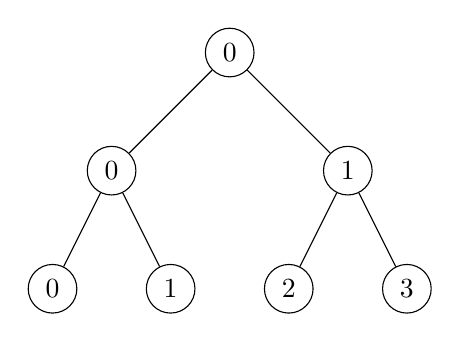
\begin{tikzpicture}[level/.style={sibling distance=30mm/#1}]
        \node [circle, draw] (a) {$0$}
            child {
                node [circle,draw] (b) {$0$}
                    child {
                        node [circle,draw] (d) {$0$}
                    }
                    child {
                        node [circle,draw] (e) {$1$}
                    }
            }
            child {
                node [circle,draw] (c) {$1$}
                    child {
                        node [circle,draw] (f) {$2$}
                    }
                    child {
                        node [circle,draw] (g) {$3$}
                    }
            };
    \end{tikzpicture}
    \end{minipage}
    \begin{minipage}[b]{.5\linewidth}
    \centering
    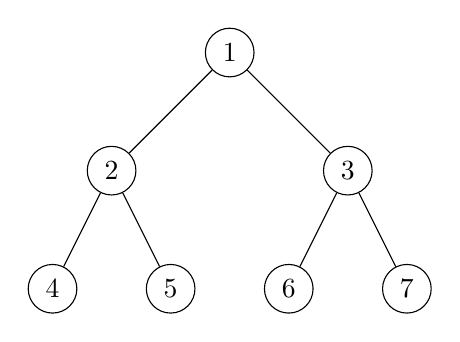
\begin{tikzpicture}[level/.style={sibling distance=30mm/#1}]
        \node [circle, draw] (a) {$1$}
            child {
                node [circle,draw] (b) {$2$}
                    child {
                        node [circle,draw] (d) {$4$}
                    }
                    child {
                        node [circle,draw] (e) {$5$}
                    }
            }
            child {
                node [circle,draw] (c) {$3$}
                    child {
                        node [circle,draw] (f) {$6$}
                    }
                    child {
                        node [circle,draw] (g) {$7$}
                    }
            };
    \end{tikzpicture}
    \end{minipage}
    \caption{Rappresentazione di due alberi di proliferazione, le cui radici
        rappresentano le cellule appartenenti alla popolazione iniziale $X_{0}$
        mentre ogni livello comprende nodi raffiguranti cellule appartenenti
        a nuove popolazioni cellulari}
    \label{fig:prolif-tree}
\end{figure}
In figura \ref{fig:prolif-tree} sono raffigurati due alberi di proliferazione,
dove ogni nodo
rappresenta l'indice di una cellula all'interno dell'array della popolazione
corrispondente al livello degli alberi considerato, come segue:

\begin{itemize}
    \item $X_{0} = [0, 1]$
    \item $X_{1} = [0, 1, 2, 3]$
    \item $X_{2} = [0, 1, 2, 3, 4, 5, 6, 7]$    
\end{itemize}

Si denoti con $B_{i,j}$ un generico thread block dove
$i$ rappresenta la popolazione $X_{i}$, mentre $j$ l'indice del blocco.
Quindi $B_{0,0} = \{0, 1\}$ sarà il blocco che date le
cellule $\{0, 1\} \subseteq X_{0}$ si occupa di
computare le figlie risultanti dalla divisione, ovvero
$\{0, 1, 2, 3\} \subseteq X_{1}$.
Al termine della computazione di $B_{0,0}$, viene invocata la primitiva 
\textit{\_\_syncthreads()} ed eseguito un nuovo Kernel, che istanzierà
i blocchi $B_{1,0} = \{0, 1\}$ e $B_{1,1} = \{2, 3\}$, che a loro volta
eseguiranno $B_{2,0} = \{0, 1\}$, $B_{2,1} = \{2, 3\}$,
$B_{2,2} = \{4, 5\}$ e $B_{2,3} = \{6, 7\}$.
\\
Questo metodo accelera di molto l'esecuzione dell'algoritmo, ma introduce un
ulteriore problema: non è possibile conoscere ad inizio simulazione la
profondità esatta degli alberi di proliferazione necessaria a garantire lo
svolgimento di tutti i fenomeni di divisione cellulare, dato che si tratta di
una simulazione di tipo stocastico.
\\
Un altro problema che è sorto è la limitazione hardware del parallelismo
dinamico, dettata dal fatto che è possibile utilizzare solamente un massimo
di 24 livelli di ricorsione. Questo limite ci costringe a dover
eventualmente terminare la computazione di alcune popolazioni cellulari qualora
rappresentino un livello di proliferazione superiore alla limitazione hardware,
iterando nuovamente come se $X_{n}$ rappresentasse una nuova
popolazione iniziale $X_{0}$ ino a raggiungere il termine della simulazione.

\begin{figure}[t]
    \centering
    \begin{tikzpicture}
        \begin{axis}[legend pos=outer north east,
                xtick=data,
                xlabel={$\tau_{max}$},
                ylabel={tempo simulazione (s)}
            ]
            \addplot table[x=Time, y=Original] {Data/Accelerants/fit.txt};
            \addplot table[x=Time, y=Dynamic] {Data/Accelerants/fit.txt};
            \legend{Senza acceleranti, Parallelismo dinamico}
        \end{axis}
    \end{tikzpicture}
    \caption{Confronto dei tempi di esecuzione (in secondi) dell'algoritmo
    parallelo fra la prima versione senza acceleranti e la versione
    che implementa il parallelismo dinamico, utilizzando differenti valori di
    tempo massimo di proliferazione $\tau_{max}$}
    \label{chart:original-dynamic}
\end{figure}
Dal grafico in figura \ref{chart:original-dynamic} è possibile vedere
l'aumento significativo delle
performance rispetto alla versione che non presenta l'utilizzo del
parallelismo dinamico. Questo è dovuto al fatto che la
sincronizzazione di tutti i blocchi della GPU effettuata al termine di ogni
iterazione e il trasferimento
dei dati da GPU a CPU per l'aggiornamento dell'array dei risultati sono
particolarmente onerosi.

% Descrizione del metodo di bound
\paragraph{Bounding}\mbox{}
\\
Sebbene il parallelismo dinamico introduca un enorme vantaggio, porta con sè
una limitazione importante, ovvero il fatto che un Kernel non termina la sua
esecuzione fino a quando tutti i Kernel invocati da quest'ultimo non sono
anch'essi terminati. Durante la computazione degli alberi questo può portare
ad alcuni rallentamenti, poiché è inutile computare rami le cui cellule
sono state marcate come $Inactive$ o $Remove$ dato che non contribuiscono
alla creazione del nuovo livello di proliferazione.
Utilizzando la Shared Memory\cite{sanders2010cuda}
, ovvero una zona di memoria condivisa tra tutti e soli i thread appartenenti ad
uno stesso thread block, è possibile
settare un flag indicante l'avvenuto evento di proliferazione
cellulare. Se ci si trovasse nel caso in cui nessun evento si è verificato,
sarebbe inutile invocare un nuovo Kernel, di conseguenza
la computazione dei successivi sotto-alberi viene interrotta per consentire
la preventiva terminazione dei Kernel precedenti.
\\
Siano $A = Alive$, $I = Inactive$, $R = Remove$, allora il metodo implementato
produce i risultati rappresentati in figura \ref{fig:tree-bounding}.
Come è possibile notare,
l'albero risultante dall'applicazione del
bounding presenta un numero inferiore nodi, ciò equivale al fatto di risparmiare
risorse evitando la computazione di sotto-alberi inutili ai fini della
simulazione.

\begin{figure}[t]
\begin{minipage}[b]{.5\linewidth}
\centering
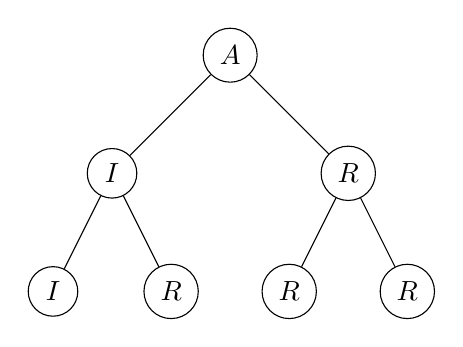
\begin{tikzpicture}[level/.style={sibling distance=30mm/#1}]
    \node [circle, draw] (a) {$A$}
        child {
            node [circle,draw] (b) {$I$}
                child {
                    node [circle,draw] (d) {$I$}
                }
                child {
                    node [circle,draw] (e) {$R$}
                }
        }
        child {
            node [circle,draw] (c) {$R$}
                child {
                    node [circle,draw] (f) {$R$}
                }
                child {
                    node [circle,draw] (g) {$R$}
                }
        };
\end{tikzpicture}
\subcaption{Senza bounding}
\end{minipage}
\begin{minipage}[b]{.5\linewidth}
\centering
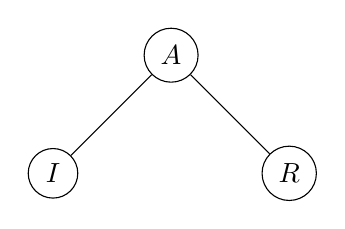
\begin{tikzpicture}[level/.style={sibling distance=30mm/#1}]
    \node [circle, draw] (a) {$A$}
        child {
            node [circle,draw] (b) {$I$}
        }
        child {
            node [circle,draw] (c) {$R$}
        };
\end{tikzpicture}
\subcaption{Bounding}
\end{minipage}
\caption{Confronto di alberi di proliferazione cellulare utilizzando il metodo
    del bounding}
\label{fig:tree-bounding}
\end{figure}
\begin{figure}[t]
    \centering
    \begin{tikzpicture}
        \begin{axis}[legend pos=outer north east,
                xtick=data,
                xlabel={$\tau_{max}$},
                ylabel={tempo simulazione (s)}
            ]
            \addplot table[x=Time, y=Dynamic] {Data/Accelerants/fit.txt};
            \addplot table[x=Time, y=Bounding] {Data/Accelerants/fit.txt};
            \legend{Parallelismo, Bounding}
        \end{axis}
    \end{tikzpicture}
    \caption{Confronto dei tempi di esecuzione (in secondi) dell'algoritmo
    parallelo fra la versione che implementa solamente il parallelismo dinamico
    e la versione che oltre a quest'ultimo fa uso anche del metodo del bounding,
    utilizzando differenti valori di tempo massimo di proliferazione
    $\tau_{max}$}
    \label{chart:dynamic-bounding}
\end{figure}
In entrambe la versioni dell'algoritmo mostrate nel grafico in figura
\ref{chart:dynamic-bounding} si nota che il tempo di simulazione
rimane costante anche al crescere del limite $\tau_{max}$ grazie al parallelismo
dinamico implementato in precedenza.
Il leggero aumento delle prestazioni mostrato in figura
\ref{chart:dynamic-bounding} indica che la tecnica
del bounding ha poco impatto sull'aumento delle performance, ma
sicuramente contribuisce alla migliore gestione delle risorse computazionali
relative alla GPU e all'uso intensivo del parallelismo dinamico. Infatti
quando un kernel padre invoca un kernel figlio,
il padre dovrà attendere la fine di tutti i suoi kernel figli per
poter procedere con l'esecuzione del codice e terminare a sua volta.
Questa tecnica di bounding risulterà molto più utile in seguito, con
l'implementazione dell'ultimo accelerante.

% Descrizione del metodo di inferenza della profondità dell'albero
\paragraph{Inferenza del livello di profondità}\mbox{}
\\
Sebbene CUDA ci ponga un livello massimo di nesting pari a 24 livelli,
nei modelli presi in considerazione per queste simulazioni, difficilmente
viene superata la soglia dei $5$ eventi di proliferazione per ogni cellula,
ma la versione dell'algoritmo dopo l'implementazione del parallelismo dinamico
prevede l'allocazione di $N$ livelli di proliferazione pari al numero massimo
di cellule che è possibile mantenere sulla memoria dedicata alla GPU.
Dunque se è presente sufficiente
spazio per allocare $10$ livelli di profondità essi vengono allocati,
consumando più risorse del dovuto. Non è nemmeno possibile utilizzare
la memoria di \textit{swap} dato che le GPU non supportano questa
funzionalità.
È necessario quindi trovare un modo per inferire nel modo più accurato
possibile il numero di livelli necessari alla simulazione.
Un modo banale potrebbe essere quello di dare la possibilità all'utente di
specificare il numero di livelli da utilizzare durante la simulazione,
a patto che sia al corrente del numero medio di divisioni necessarie per ogni cellula
appartenente ad $X_{0}$ al fine di portare a termine la simulazione.
Un altro metodo risulta essere la possibilità di inferire il numero dei livelli
necessari utilizzando i parametri forniti in ingresso alla simulazione.
Per poter calcolare i diversi tipi di cellule, si utilizza un array di
parametri contenente le distribuzioni uniformi $\pi$ dei vari tipi di cellule
$\tau$ che è possibile avere all'interno della popolazione iniziale.
Ogni tipo di cellula possiede un tempo medio $\mu$ dopo il quale avviene
la divisione, il quale segue una distribuzione normale.
È possibile pensare di utilizzare il tempo medio $\mu_{i}$ del tipo di cellula
$\tau_{i}$ che ha probabilità $\pi_{i}$ maggiore per calcolare un numero
approssimativo di livello di divisioni tali per cui venga superato il
$\tau_{max}$ definito per la simulazione.
\\
Sia $\mu_{max}$ il tempo medio di divisione
del tipo di cellula avente $max(\pi)$.
Allora è possibile stimare che il numero $\eta$ dei livelli di profondità
dell'albero è dato dalla seguente relazione
$$\eta : \sum\limits_{i=1}^{\eta - 1}
\mu_{max} \leqslant \tau_{max} \leqslant \sum\limits_{i=1}^{\eta} \mu_{max}$$

Questo valore è utile per l'ottimizzazione del numero di livelli necessario
per portare a termine la simulazione mediante una sola iterazione.
Essendo però un processo di tipo stocastico, è possibile che il valore calcolato
$\eta$ non rispecchi a pieno la realtà che si vuole simulare.

\begin{figure}[t]
    \centering
    \begin{tikzpicture}
        \begin{axis}[legend pos=outer north east,
                xtick=data,
                xlabel={$\tau_{max}$},
                ylabel={tempo simulazione (s)}
            ]
            \addplot table[x=Time, y=Bounding] {Data/Accelerants/fit.txt};
            \addplot table[x=Time, y=Inference] {Data/Accelerants/fit.txt};
            \legend{Bounding, Inferenza}
        \end{axis}
    \end{tikzpicture}
    \caption{Confronto dei tempi di esecuzione (in secondi) dell'algoritmo
    parallelo fra la versione che implementa gli acceleranti descritti fino al
    metodo del bounding
    e la versione che oltre a quest'ultimo utilizza anche l'inferenza del numero
    di livelli necessari alla simulazione,
    utilizzando differenti valori di tempo massimo di proliferazione
    $\tau_{max}$}
    \label{chart:bounding-inference}
\end{figure}
Nel grafico in figura \ref{chart:bounding-inference} si può notare un
incremento di prestazioni fino
ad un valore di $\tau_{max}$ di $720$, questo perché sebbene venga applicata
l'inferenza dei parametri, l'algoritmo prevede l'istanziamento di $\eta$
livelli solamente se è disponibile abbastanza memoria all'interno della GPU.
Infatti con una valore di $\tau_{max} > 720$ non è presente nessun aumento
di prestazioni poiché la GPU utilizzata non ha abbastanza memoria per istanziare
un numero di livelli pari a $\eta$ inferito dai parametri iniziali.
Quindi risulta sicuramente un vantaggio l'utilizzo di GPU con molta memoria
dedicata a disposizione.

% Descrizione della costruzione dell'istogramma finale
\paragraph{Calcolo dell'istogramma finale}\mbox{}
\\
Sebbene le performance siano aumentate, il software fa ancora molto affidamento
sulla CPU per il calcolo dell'istogramma finale.
Ad ogni iterazione l'array della popolazione $X_{n}$ viene trasferito
attraverso la CPU in memoria centrale per essere filtrato e per aggiornare i
risultati dell'istogramma. Questo processo è possibile grazie alla funzione
\textit{cudaMemcpy()} che si occupa del trasferimento dei dati tra CPU e GPU.
Diverse chiamate a questa funzione generano un lavoro intensivo che deve essere
effettuato, quindi impatta ulteriormente sullo speedup della simulazione.
L'obiettivo è quindi cercare di minimizzare il numero di trasferimenti tramite
\textit{cudaMemcpy()}.
\\
La soluzione risiede nella possibilità di calcolare l'istogramma direttamente
sulla GPU. Assumendo di conoscere un array ordinato in modo crescente$\Omega$
contenente tutti possibili valori di fluorescenza
$\varphi$ che una cellula potrà assumere in futuro, è possibile far eseguire
ad un thread del kernel (se computando una cellula $Active$ essa non è più in
grado di proliferare) una ricerca binaria su $\Omega$ e aggiornare
il valore di frequenza $\psi$ corrispondente alla fluorescenza trovata, tramite
la funzione $atomicAdd()$ di CUDA, la quale anche se prevede una
sincronizzazione sulla risorsa a cui si vuole accedere, è necessaria dato che
ad ora non esiste un altro modo per il calcolo di un istogramma attraverso un
algoritmo parallelo.
\\
Conoscendo l'istogramma iniziale $H(0)$ si hanno già a disposizione
tutti i valori di fluorescenza che una cellula potrà assumere, infatti
$\Omega$ conterrà tutti i valori di $H(0)$ tali che $\varphi_{i} \geqslant
\varphi_{min}$ e i successivi valori $\varphi_{i}^{-2j}$ con $j \in \N, j > 0$.
\\
Questa tecnica evita il trasferimento dati al termine di ogni iterazione, poiché
la frequenza riguardante i valori di fluorescenza delle cellule $Inactive$
è già stata aggiornata durante l'esecuzione del kernel.
Mediante questa tecnica la $cudaMemcpy()$ viene utilizzata solamente a inizio
e fine simulazione per il salvataggio dei risultati.
\\
Come si evince dal grafico in figura \ref{chart:inference-histogram}, 
questo è l'accelerante che incrementa maggiormente
le performance dell'algoritmo, dato che risolve quasi totalmente il problema
del collo di bottiglia causato dal trasferimento bidirezionale delle informazioni
per l'avanzamento della simulazione.
\begin{figure}[t]
    \centering
    \begin{tikzpicture}
        \begin{axis}[legend pos=outer north east,
                xtick=data,
                xlabel={$\tau_{max}$},
                ylabel={simulation time (s)}
            ]
            \addplot table[x=Time, y=Inference] {Data/Accelerants/fit.txt};
            \addplot table[x=Time, y=Histogram] {Data/Accelerants/fit.txt};
            \legend{Inferenza, Istogramma parallelo}
        \end{axis}
    \end{tikzpicture}
    \caption{Confronto dei tempi di esecuzione (in secondi) dell'algoritmo
    parallelo fra la versione che implementa gli acceleranti descritti fino al
    metodo dell'inferenza dei parametri
    e la versione che oltre a quest'ultimo implementa anche il calcolo parallelo
    dell'istogramma finale,
    utilizzando differenti valori di tempo massimo di proliferazione
    $\tau_{max}$}
    \label{chart:inference-histogram}
\end{figure}

% Descrizione del problema della gestione della memoria
\subsection{Gestione della memoria}

L'implementazione degli acceleranti ha migliorato di gran lunga le
performance dell'algoritmo, ma ha introdotto un problema, ovvero la crescita
esponenziale della memoria.
Infatti data la numerosità $L$ della popolazione iniziale $X_{0}$, essa cresce
esponenzialmente con il numero dei livelli dell'albero $L * 2^i$ con
$i \in \N, i > 0$. Inizialmente questa crescita era mitigata dal fatto che
dopo ogni iterazione la popolazione veniva filtrata, quindi procedendo verso
il termine della simulazione, l'utilizzo di memoria veniva bilanciato dalla
poca numerosità delle cellule $Alive$ rimanenti.
Dopo l'introduzione dell'ultimo accelerante, sebbene le cellule $Inactive$ e
$Remove$ non vengano prese in considerazione per la computazione, sono
comunque presenti ancora all'interno delle diverse popolazioni, dato che
dopo ogni iterazione la memoria non viene più filtrata in quanto non più
trasferita sulla CPU.
\\
La crescita esponenziale dell'occupazione di memoria visibile in figura
\ref{chart:serial-parallel-histogram} potrebbe essere un
problema nel momento in cui il tempo $\tau_{max}$ inizia a crescere
ulteriormente. La soluzione immediata a questo problema potrebbe essere di
natura economica, ovvero l'acquisto di GPU moderne con molta memoria a
disposizione. Il problema però persiste, quindi una possibile soluzione
potrebbe essere quella di computare ad un certo punto solamente un sottoinsieme
della popolazione e trasferire i restanti elementi sulla CPU, per poi
elaborarli nuovamente quando il primo sottoinsieme di popolazione è stato
elaborato. Questo però introdurrebbe nuovamente la necessità di utilizzare
in modo assiduo $cudaMemcpy()$, però fino ad ora pare essere l'unica soluzione
plausibile.

\begin{figure}[t]
    \centering
    \begin{tikzpicture}
        \begin{axis}[legend pos=north west,
                xtick=data,
                xlabel={iterazioni dell'algoritmo},
                ylabel={dimensione popolazione (MB)}
            ]
            \addplot table[x=Iteration, y=Serial] {Data/Memory/validation.txt};
            \addplot table[x=Iteration, y=Parallel] {Data/Memory/validation.txt};
            \legend{Istogramma seriale,Istogramma parallelo}
        \end{axis}
    \end{tikzpicture}
    \caption{Confronto dell'utilizzo di memoria fra la versione dell'algoritmo
        che prevede il calcolo seriale dell'istogramma con rimozione delle
        cellule non $Alive$ e il calcolo parallelo dell'istogramma dei risultati
        senza filtraggio della popolazione cellulare al termine di $n$ iterazioni
        dell'algoritmo}
    \label{chart:serial-parallel-histogram} 
\end{figure}
